\documentclass{beamer}
\usetheme{Madrid}
\usecolortheme{default}
\usepackage{amsmath}
\usepackage{tikz}
\usepackage{}
\usetikzlibrary{arrows.meta}

\title{Relative Motion}
\subtitle{SPH3UI - Day 1}
\author{}
\date{}

\begin{document}

\begin{frame}
\titlepage
\end{frame}

\begin{frame}{Relative Motion}
\begin{center}
\Large Everything is moving, but relative to what?
\end{center}
\end{frame}

\begin{frame}{How to record motion of a ball being tossed?}

\begin{figure}
  \centering
  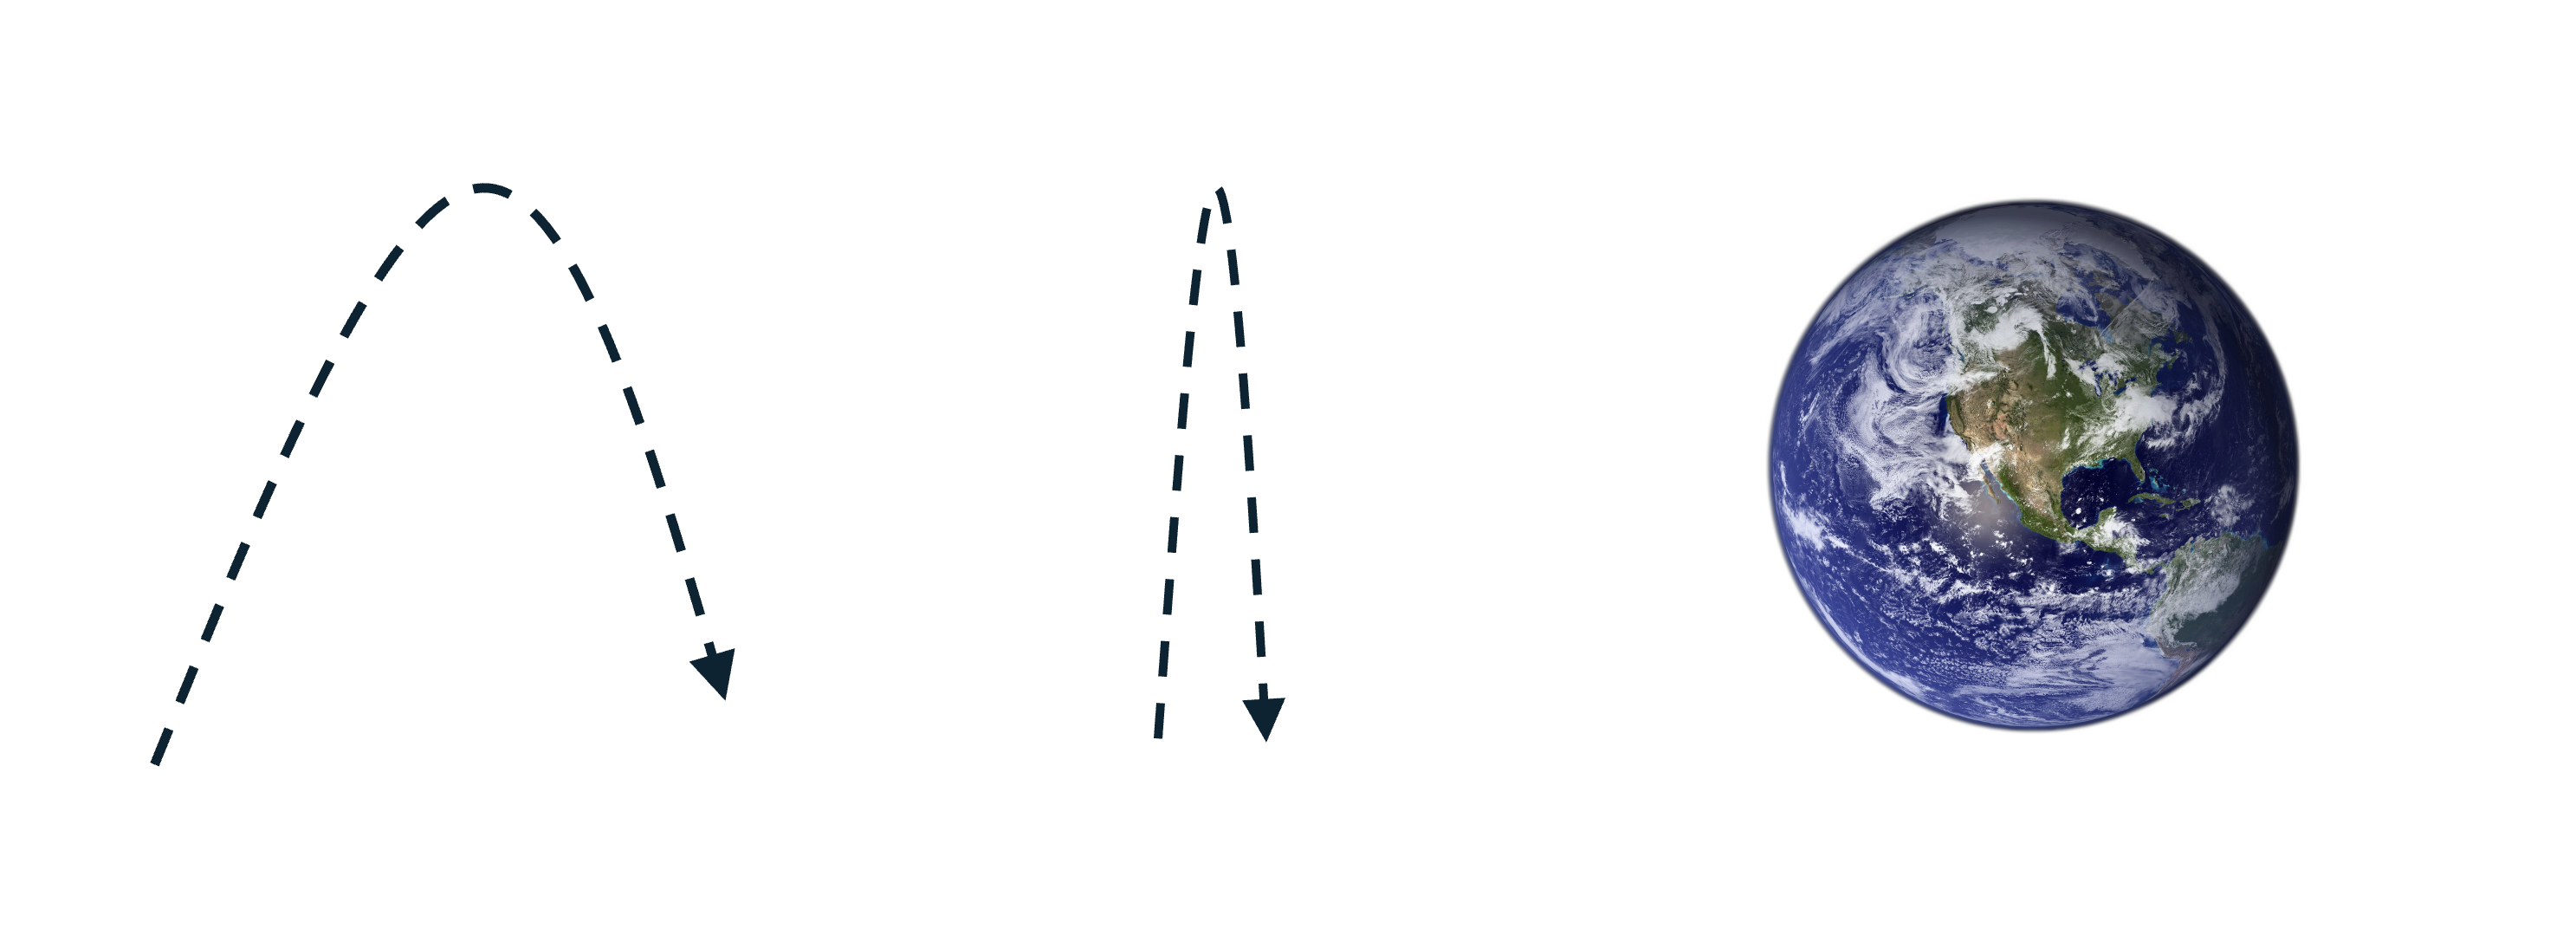
\includegraphics[width=1\textwidth]{demojpg.png}
  \label{fig:sample}
\end{figure}

*the eastward tangential velocity of Earth's surface is \(\sim 1670\) km/h at the equator
\end{frame}

\begin{frame}{Example 1: Train Station Observers}
Suppose two people are observing each other at a train station.

\vspace{0.3cm}

Observer A stands stationary on the station platform while Observer B is seated on a train moving east at 20 km/h.

\vspace{0.5cm}

\begin{center}
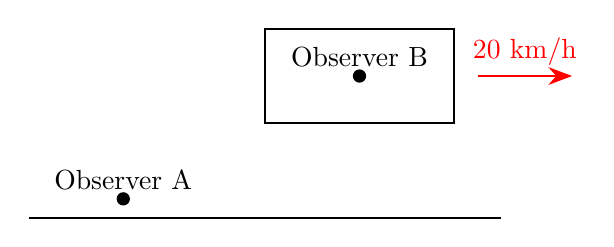
\begin{tikzpicture}[scale=1.2]
% Platform
\draw[thick] (0,0) -- (5,0);
\fill[black] (1,0.2) circle (2pt) node[above] {Observer A};
% Train
\draw[thick] (2.5,1) rectangle (4.5,2);
\fill[black] (3.5,1.5) circle (2pt) node[above] {Observer B};
\draw[-{Stealth[length=3mm]}, thick, red] (4.75,1.5) -- (5.75,1.5) node[midway, above] {20 km/h};
\end{tikzpicture}
\end{center}

\vspace{0.3cm}

\end{frame}

\begin{frame}{Example 1: Questions}
\textbf{a) What is the velocity of Observer B according to Observer A?}


\[\vec{v}_{BA} = 20 \text{ km/h [E]}\]



\textbf{b) What is the velocity of Observer A according to Observer B?}


\[\vec{v}_{AB} = 20 \text{ km/h [W]} = -20 \text{km/h}[E]\]



\textbf{c) What is the relationship between velocities of these different observers?}


\[\vec{v}_{AB} = -\vec{v}_{BA}\]
\end{frame}

\begin{frame}{Key Concept}
The laws of physics that apply when you are at rest relative to the Earth also apply when you are in any reference frame moving at constant velocity relative to the Earth.

\vspace{0.5cm}

Motion may look different depending on the reference frame of the observer, but we can describe this relationship mathematically by including the relative velocity of the reference frame in the description of the motion.
\end{frame}

\begin{frame}{Relative Velocity Formula}
\[\vec{v}_{BA} = \vec{v}_{BT} + \vec{v}_{TA}\]

\vspace{0.5cm}

To describe motion in one reference frame according to an observer in another reference frame, we determine a common reference frame:

\vspace{0.3cm}

\begin{itemize}
\item \(\vec{v}_{BA}\) = Velocity of Observer B, according to Observer A
\item \(\vec{v}_{BT}\) = Velocity of Observer B relative to the train
\item \(\vec{v}_{TA}\) = Velocity of the train relative to observer A
\end{itemize}
\end{frame}

\begin{frame}{Example 1d}
\textbf{d) If Observer B starts walking towards the front of the train at 5 km/h, how would Observer A describe the velocity of Observer B?}



\textbf{Given:}
\begin{itemize}
\item \(\vec{v}_{BT} = 5\) km/h [E] (walking forward)
\item \(\vec{v}_{TA} = 20\) km/h [E] (train velocity)
\end{itemize}



\textbf{Solution:}
\[\vec{v}_{BA} = \vec{v}_{BT} + \vec{v}_{TA}\]

\[= 5 \text{ km/h [E]} + 20 \text{ km/h [E]}\]

\[= 25 \text{ km/h [E]}\]
\end{frame}

\begin{frame}{Example 2: Minivan and Prius}
Consider the motion of a Minivan and a Prius, moving at 13 mi/h and 34 mi/h towards the East, respectively.

\vspace{0.5cm}

\begin{center}
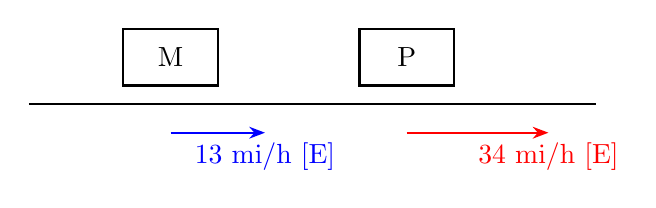
\begin{tikzpicture}[scale=1.2]
% Road
\draw[thick] (0,0) -- (6,0);
% Minivan
\draw[thick] (1,0.2) rectangle (2,0.8);
\node at (1.5,0.5) {M};
\draw[-{Stealth[length=2mm]}, thick, blue] (1.5,-0.3) -- (2.5,-0.3) node[below] {13 mi/h [E]};
% Prius
\draw[thick] (3.5,0.2) rectangle (4.5,0.8);
\node at (4,0.5) {P};
\draw[-{Stealth[length=2mm]}, thick, red] (4,-0.3) -- (5.5,-0.3) node[below] {34 mi/h [E]};
\end{tikzpicture}
\end{center}

\vspace{0.3cm}

\textbf{a) If you are driving the Prius and look out the window to see the minivan go by, how fast would you observe the minivan to be moving?}



\textbf{b) If you are driving the minivan, how fast would you observe the Prius to be moving?}
\end{frame}

\begin{frame}{Example 2: Solution Part a}

\href{https://youtu.be/jYMU6bn5GHY?si=V_nLU3Sra3oxjf_y}{Video: \textit{Introduction to Relative Motion using a Quadcopter Drone (UAV) by Flipping Physics}}
\vspace{0.3cm}

\textbf{a) Velocity of minivan according to Prius driver}



\textbf{Given:}
\begin{itemize}
\item \(\vec{v}_{MG} = 13\) mi/h [E] (minivan relative to ground)
\item \(\vec{v}_{PG} = 34\) mi/h [E] (Prius relative to ground)
\end{itemize}



\textbf{Analysis:}
\[\vec{v}_{MP} = \vec{v}_{MG} - \vec{v}_{PG}\]



\textbf{Solution:}
\[\vec{v}_{MP} = 13 \text{ mi/h [E]} - 34 \text{ mi/h [E]}\]

\[= -21 \text{ mi/h [E]} = 21 \text{ mi/h [W]}\]
\end{frame}

\begin{frame}{Example 2: Solution Part b}
\textbf{b) Velocity of Prius according to minivan driver}



\textbf{Analysis:}
\[\vec{v}_{PM} = \vec{v}_{PG} - \vec{v}_{MG}\]



\textbf{Solution:}
\[\vec{v}_{PM} = 34 \text{ mi/h [E]} - 13 \text{ mi/h [E]}\]

\[= 21 \text{ mi/h [E]}\]



\vspace{0.5cm}

\textbf{Note:} \(\vec{v}_{PM} = -\vec{v}_{MP}\)
\end{frame}

\begin{frame}{Example 3: Plane in Wind}
A pilot flies their plane so that their compass reads 'South' with an airspeed (i.e., the speed of the plane relative to the molecules in the air) of 200 km/h.

There is a wind blowing from the South at 40 km/h.

\begin{center}
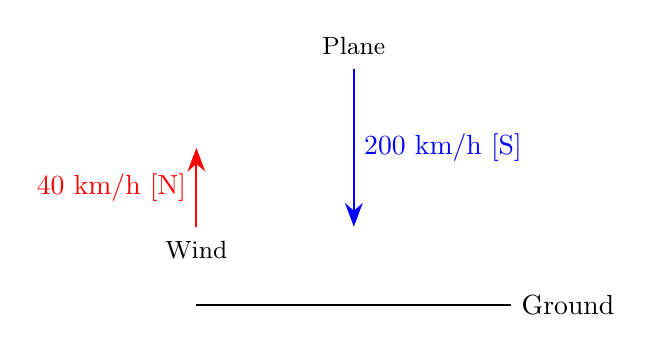
\begin{tikzpicture}[scale=1.0]
% Plane velocity
\draw[-{Stealth[length=3mm]}, thick, blue] (2,3) -- (2,1) node[midway, right] {200 km/h [S]};
\node at (2,3.3) {\small Plane};
% Wind velocity
\draw[-{Stealth[length=3mm]}, thick, red] (0,1) -- (0,2) node[midway, left] {40 km/h [N]};
\node at (0,0.7) {\small Wind};
% Ground
\draw[thick] (0,0) -- (4,0) node[right] {Ground};
\end{tikzpicture}
\end{center}

\textbf{a) What is the velocity of the plane relative to the ground?}

\textbf{b) How long will it take the plane to travel 500 km [S] relative to the ground?}
\end{frame}

\begin{frame}{Example 3: Solution Part a}
\textbf{a) What is the velocity of the plane relative to the ground?}



\textbf{Given:}
\begin{itemize}
\item \(\vec{v}_{PA} = 200\) km/h [S] (plane relative to air)
\item \(\vec{v}_{AG} = 40\) km/h [N] (air/wind relative to ground)
\end{itemize}



\textbf{Analysis:}
\[\vec{v}_{PG} = \vec{v}_{PA} + \vec{v}_{AG}\]



\textbf{Solution:}
\[\vec{v}_{PG} = 200 \text{ km/h [S]} + 40 \text{ km/h [N]}\]

\[= 200 \text{ km/h [S]} - 40 \text{ km/h [S]}\]

\[= 160 \text{ km/h [S]}\]
\end{frame}

\begin{frame}{Example 3: Solution Part b}
\textbf{b) How long will it take the plane to travel 500 km [S] relative to the ground?}



\textbf{Given:}
\begin{itemize}
\item \(\vec{v}_{PG} = 160\) km/h [S]
\item \(\Delta d = 500\) km [S]
\end{itemize}



\textbf{Analysis:}
\[\vec{v}_{PG} = \frac{\Delta \vec{d}}{\Delta t} \Rightarrow \Delta t = \frac{\Delta \vec{d}}{\vec{v}}\]



\textbf{Solution:}
\[\Delta t = \frac{500 \text{ km}}{160 \text{ km/h}}\]

\[= 3.125 \text{ h} = 3 \text{ h } 7.5 \text{ min}\]
\end{frame}

\begin{frame}{What did we learn?}

\href{https://youtu.be/wD7C4V9smG4?si=9NaAkSsVkEW4FQBZ}{Video: \textit{Professor Dave Explains Relative Motion}}


\begin{itemize}
\item Motion is always relative. There is no "absolute rest", only motion relative to something else.



\item Laws of physics don't change between observers moving at constant velocity. E.g., tossing a ball will look the same on the bus as on the ground.



\item Different observers describe motion differently, but their observations can be related by finding a common reference frame.



\item \textbf{Notation convention:} The first subscript represents the object, and the second subscript represents the observer. E.g., \(\vec{v}_{BA}\) means velocity of object B as seen by observer A.



\item \textbf{Key formula:} \(\vec{v}_{BA} = \vec{v}_{BT} + \vec{v}_{TA}\)
\end{itemize}
\end{frame}

\begin{frame}{Practice Extension: Walking on a Conveyor Walkway}

\textbf{Scenario:}  
A traveler is stuck in the airport and decides to get some exercise. They walk at a constant speed of 1.5 m/s relative to the conveyor walkway. The walkway itself moves at 2.0 m/s relative to the ground.

\vspace{0.4cm}

\textbf{(a)}
If the traveler walks \emph{against} the motion of the walkway (i.e., toward the back while the walkway moves forward):
\begin{itemize}
    \item Interpret the traveler’s velocity relative to the ground (magnitude and direction).
\end{itemize}

\vspace{0.4cm}

\textbf{(b)} Now the traveler turns around and walks \emph{with} the motion of the walkway.
\begin{itemize}
    \item Determine the new velocity of the traveler relative to the ground.
    \item How long does it take to cover 45 m walkway length in this case? Compare this to how long it would have taken without the conveyor. 
\end{itemize}

\end{frame}
\begin{frame}{Investigation: River Crossing Problem}


\vspace{0.4cm}

\textbf{River Crossing (2D Relative Motion)}  
A boat travels at 5.0 m/s [S] relative to the water. The river flows at 3.0 m/s [E].  
\begin{itemize}
    \item Find the boat’s velocity relative to the ground.
    \item Compute the resultant speed and direction (angle south of east).
    \item Sketch the velocity vector diagram.
\end{itemize}

\end{frame}


\end{document}
